% Appendix: additional generated tables and figures.

\subsection{Unambiguous synthetic subset}
Synthetic clouds that a simpler family also fits equally well (judged from B1's per-family fits) are tagged ambiguous (\ambiguousFrac{} of the baseline subset). Table~\ref{tab:unambiguous} repeats Table~\ref{tab:results} without them.
\begin{table}[H]
\centering
\caption{Systems on the baseline subset without ambiguous clouds.}
\label{tab:unambiguous}
\resizebox{\textwidth}{!}{\scriptsize
\begin{tabular}{lllllllll}
\toprule
\textbf{System} & \textbf{n} & \textbf{Fine accuracy [95\% CI]} & \textbf{Macro-F1 [95\% CI]} & \textbf{Coarse accuracy} & \textbf{Superset-OK accuracy} & \textbf{Median Chamfer to GT [95\% CI]} & \textbf{Mean residual} & \textbf{Median axis error (deg)} \\
\midrule
Method (network + refinement) & 2060 & 94.0\% [93.0, 95.0] & 0.922 [0.908, 0.935] & 96.4\% & 94.3\% & 0.119 [0.111, 0.127] & 0.091 & 0.7 \\
A3: no refinement & 2060 & 94.0\% [93.0, 95.0] & 0.922 [0.908, 0.935] & 96.4\% & 94.3\% & 0.127 [0.119, 0.132] & 0.101 & 1.1 \\
A5: G-AIC selection & 2060 & 72.0\% [70.1, 74.0] & 0.654 [0.637, 0.671] & 81.5\% & 76.5\% & 0.138 [0.134, 0.144] & 0.097 & 0.6 \\
A5: hybrid selection & 2060 & 92.6\% [91.4, 93.7] & 0.902 [0.888, 0.916] & 94.8\% & 93.1\% & 0.119 [0.111, 0.128] & 0.090 & 0.7 \\
B1: classical fit + G-AIC & 2060 & 69.7\% [67.6, 71.6] & 0.636 [0.615, 0.654] & 82.5\% & 75.4\% & 0.154 [0.147, 0.160] & 0.103 & 0.6 \\
B2: features + boosting & 2060 & 72.3\% [70.3, 74.2] & 0.697 [0.674, 0.715] & 92.5\% & 76.2\% & 0.152 [0.147, 0.159] & 0.099 & 0.6 \\
B3a: always blob & 2060 & 4.5\% [3.6, 5.4] & 0.007 [0.005, 0.008] & 4.5\% & 4.5\% & 0.523 [0.517, 0.529] & 0.119 & 10.2 \\
B3b: always arc (B1 arc fit) & 2060 & 7.3\% [6.2, 8.5] & 0.011 [0.009, 0.012] & 36.3\% & 7.3\% & 0.528 [0.516, 0.538] & 0.273 & 0.3 \\
B3c: random shape & 2060 & 8.3\% [7.2, 9.5] & 0.079 [0.068, 0.090] & 34.1\% & 11.6\% & 1.114 [1.092, 1.138] & 0.582 & 58.6 \\
\bottomrule
\end{tabular}
}
\end{table}

\subsection{Training, confusion and calibration}
\begin{figure}[H]
\centering
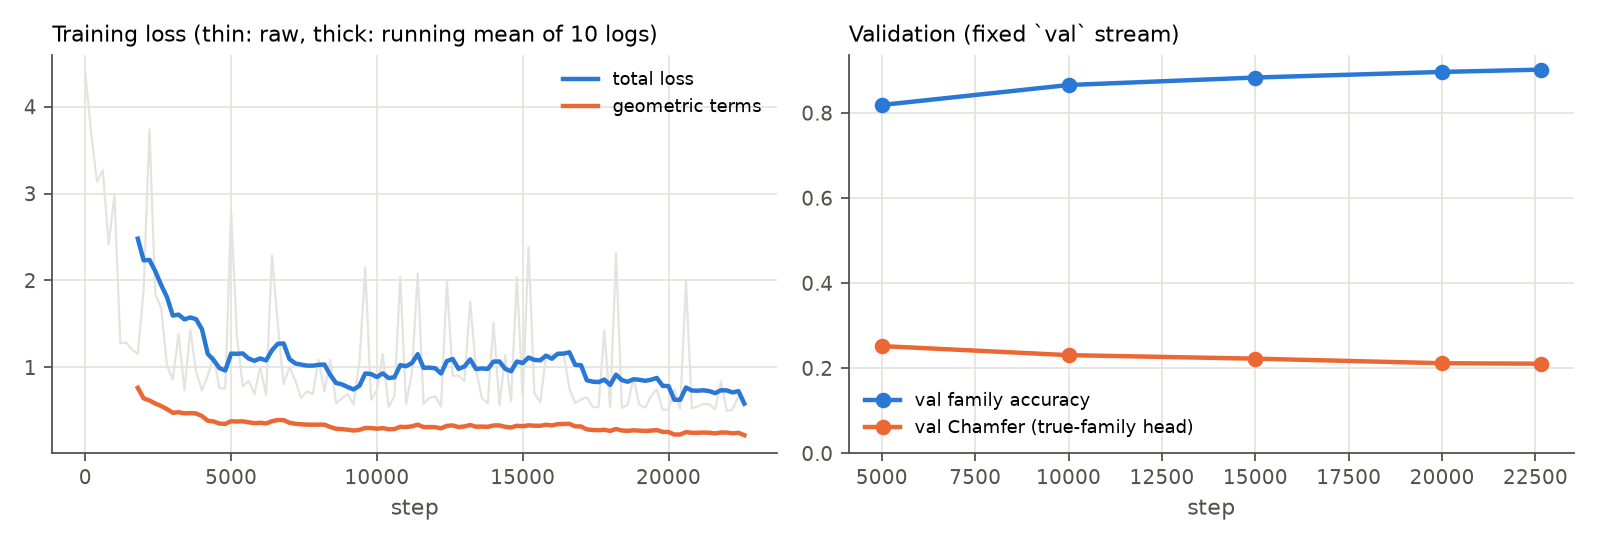
\includegraphics[width=\textwidth]{fig_training.png}
\caption{Training loss (left) and validation family accuracy and teacher-forced Chamfer distance on the fixed validation stream (right). Steps 0--9999 of the loss curve were recovered from the log of the crashed first attempt (\texttt{reports/deviations.md}).}
\label{fig:training}
\end{figure}
\begin{figure}[H]
\centering
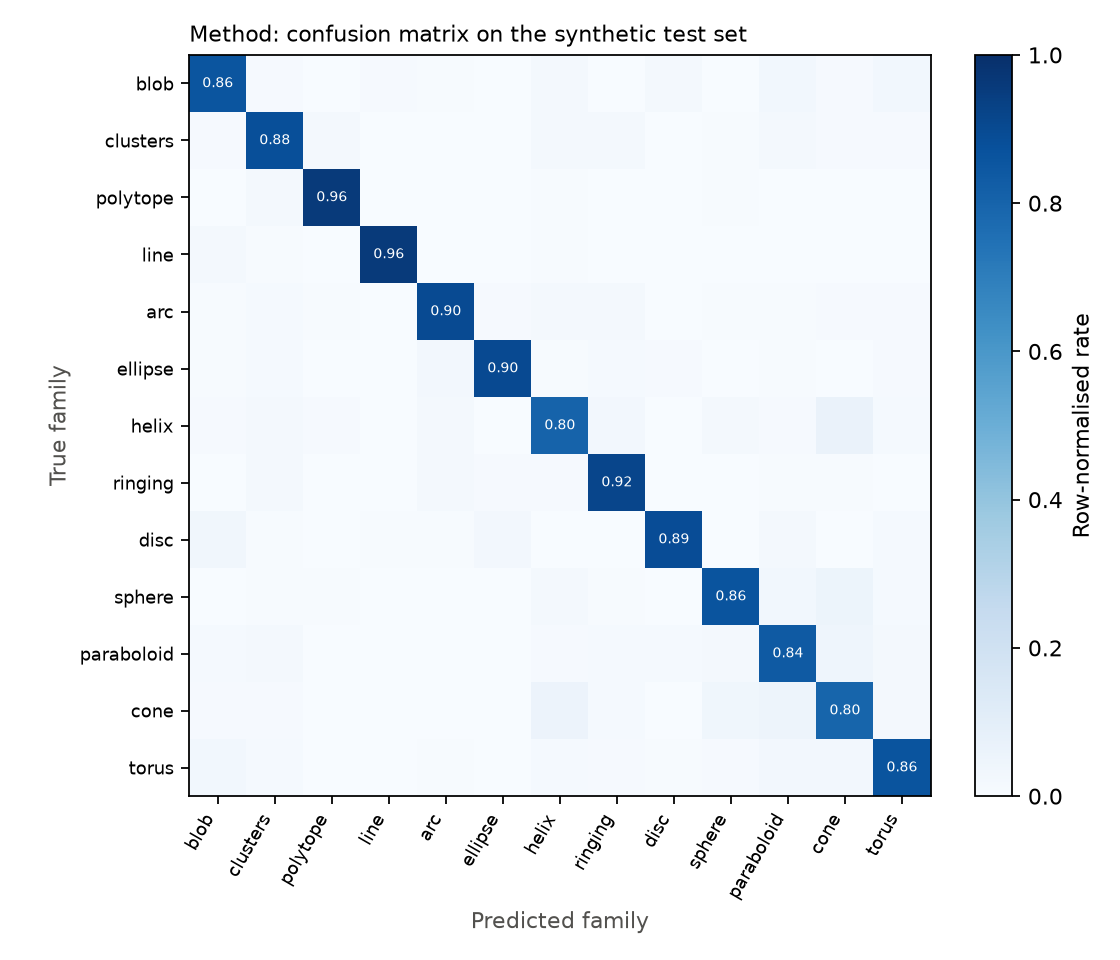
\includegraphics[width=0.55\textwidth]{fig_confusion.png}\hfill
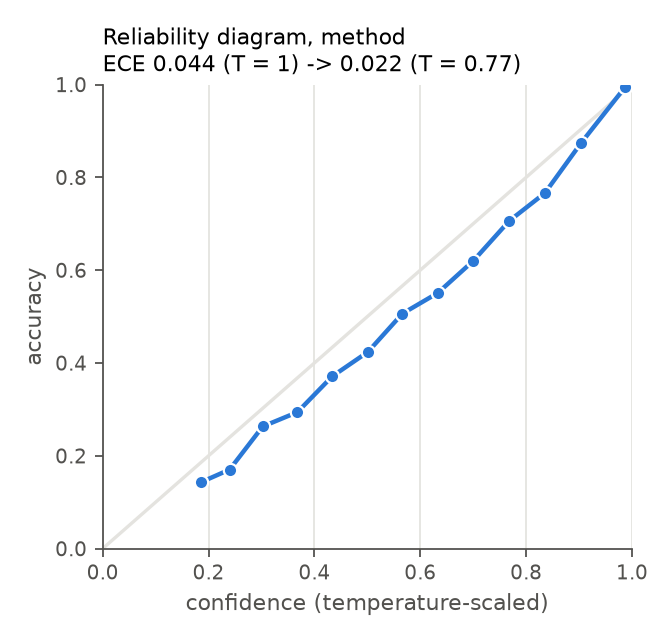
\includegraphics[width=0.4\textwidth]{fig_reliability.png}
\caption{Left: confusion matrix of the method on the full synthetic test set (row-normalised). Right: reliability diagram after temperature scaling.}
\label{fig:confusion}\label{fig:reliability}
\end{figure}
\begin{figure}[H]
\centering
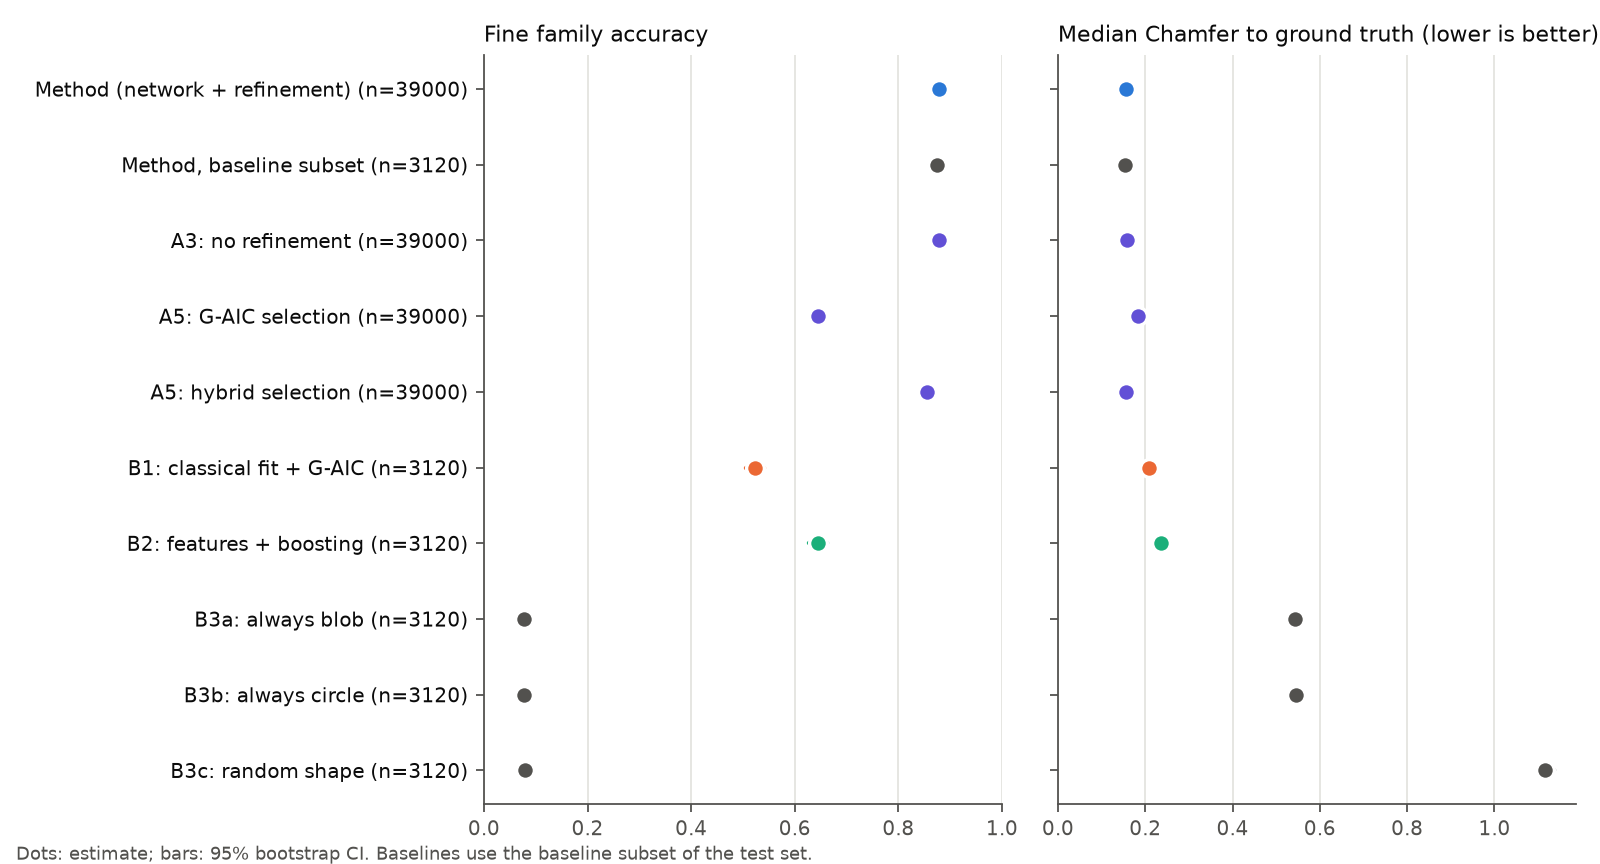
\includegraphics[width=\textwidth]{fig_systems.png}
\caption{Fine accuracy and median Chamfer distance of all systems with 95\% bootstrap CIs.}
\label{fig:systems}
\end{figure}

\subsection{Models}
\begin{table}[H]
\centering
\caption{Trained fitters.}
\resizebox{\textwidth}{!}{\scriptsize
\begin{tabular}{llllllllll}
\toprule
\textbf{Run} & \textbf{Encoder} & \textbf{Training objective} & \textbf{Data / curriculum} & \textbf{Params} & \textbf{Steps} & \textbf{Minutes} & \textbf{Val. accuracy} & \textbf{Test fine accuracy} & \textbf{Test median Chamfer} \\
\midrule
main\_s0 & Set Transformer & CE + Chamfer + residual + aux & full synthetic mix & 1,712,093 & 22643 & 110 & 90.2\% & 87.9\% & 0.156 \\
\bottomrule
\end{tabular}
}
\end{table}
